%% LaTeX Beamer presentation template (requires beamer package)
%% see http://bitbucket.org/rivanvx/beamer/wiki/Home
%% idea contributed by H. Turgut Uyar
%% template based on a template by Till Tantau
%% this template is still evolving - it might differ in future releases!

\documentclass{beamer}

\mode<presentation>
{
\usetheme{Darmstadt}

\setbeamercovered{transparent}
} 

\usepackage[english]{babel}
\usepackage[latin1]{inputenc}

% font definitions, try \usepackage{ae} instead of the following
% three lines if you don't like this look
\usepackage{mathptmx}
\usepackage[scaled=.80]{helvet}
\usepackage{courier}
\usepackage{graphicx}
\usepackage{subfigure}
\DeclareGraphicsExtensions{.pdf,.png,.jpg}


\usepackage[T1]{fontenc}


\title{Taking Multi-Object Tracking to the Next Level: People, Unknown Objects, and Carried Items}

%\subtitle{}

% - Use the \inst{?} command only if the authors have different
%   affiliation.
%\author{F.~Author\inst{1} \and S.~Another\inst{2}}
\author{Review by Igor Bogoslavskyi}

% - Use the \inst command only if there are several affiliations.
% - Keep it simple, no one is interested in your street address.
\institute[Universities of]
{
Department Of Computer Science\\
Albert Ludwigs University Freiburg\\
e-mail: bogoslai@informatik.uni-freiburg.de}

\date{2.02.2013}

\begin{document}

\begin{frame}
\titlepage
\end{frame}

\section{Motivation}
%slide 1
\begin{frame}
\frametitle{Motivation} 
\begin{itemize}
  \item Tracking objects in the moving scene is an important task in mobile robotics
\end{itemize}

\begin{center}
  \includegraphics[width=8cm]{image-intro.jpg}
\end{center}

\end{frame}

% slide 2
\begin{frame}
\frametitle{} 
\begin{itemize}
  \item Previously only \emph{tracking-by-detection} approaches. These need pre-trained detector models.
  \item It is important to recognize and track other objects in peoples' surroundings.
  \item Methods that can detect and track also novel object types and learn models for them on-line are needed.
\end{itemize}
\begin{center}
  \includegraphics[width=7.5cm]{motivation_items.jpg}
\end{center}
\end{frame}

\section{Problem Description}
%slide 3
\begin{frame}
\frametitle{Problem Description} 
\begin{itemize}
  \item The problem of detecting novel objects is not trivial.
  \item To do that one has to answer an even harder question - \emph{what is an object}.
  \item This itself involves segmenting object from the video stream input.
\end{itemize}
\end{frame}


\section{Tracking-Before-Detection}
\subsection{Overview}
%slide 4
\begin{frame}
\frametitle{Tracking-Before-Detection Approach} 
\begin{itemize}
  \item Noisy stereo estimates are used to extract regions-of-interest (ROIs) in the input images and to segment them into candidate objects.
  \item Each ROI is then tracked independently in 3D.
  \item Each segmented object is then sent to an object classifier for classification into pedestrians and other objects.
\end{itemize}
\begin{center}
  	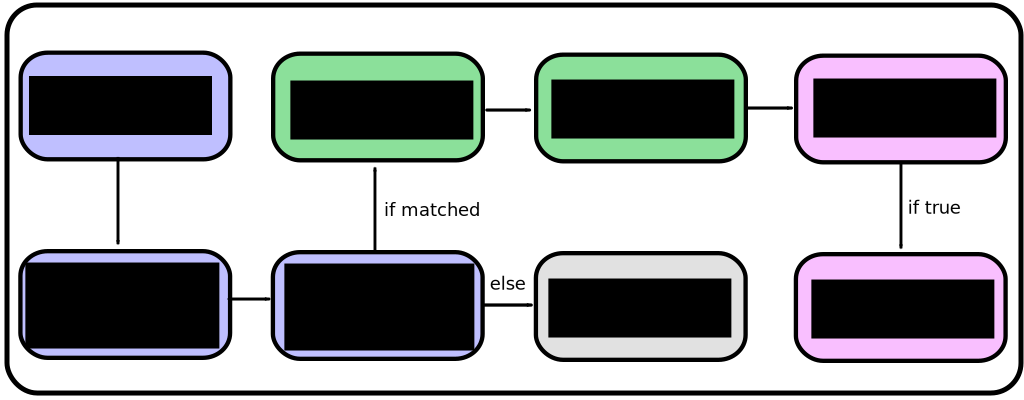
\includegraphics[width=10cm]{overview.pdf}
	\end{center}
\end{frame}

%slide 8
\subsection{3D Model}
\begin{frame}
\frametitle{3D Model Representation} 

\begin{center}
  \includegraphics[width=10cm]{3D_model.pdf}
\end{center}
\begin{itemize}
  \item The objects are represented by novel \emph{Generalized Christmas Tree} (GCT) model.
  \item The model is composed of a vertical axis and several layers of equally spaced horizontal rays.
  \item  Along each ray, 3D points are stored in distance histogram.
  \item  Representation adapts to the shape of tracked objects allowing to use median points as well as variances for better visualization. 
\end{itemize}
\end{frame}



%slide 5
\subsection{ROI Extraction and Segmentation}
\begin{frame}
\frametitle{ROI Extraction and Segmentation} 

\begin{itemize}
  \item Given depth image generate a set of ROIs for potential objects.
  \begin{itemize}
  	\item The 3D points within 2m height corridor are projected onto the ground plane.
  	\item A 2D histogram of these points is taken
  	\item The histogram bins are thresholded for removing noise.
  	\item Resulting bins are grouped into connected components (image, top)
  \end{itemize}
  \item The connected components are found by segmenting a smoothed version of the original histogram via Quick Shift algorithm.  
\end{itemize}
	\begin{center}
  \includegraphics[width=5cm]{histogram.jpg}
  \end{center}
\end{frame}

%slide 6
\subsection{Quick Shift}
\begin{frame}
\frametitle{Quick Shift} 

\begin{itemize}
  \item Quick Shift finds the modes of density by shifting each point to the nearest neighbor with higher density value. 
  %Formally:
  %$$ y_i =  \underset{j:P_j>P_i}{\operatorname{argmax}} \hspace{1pt} d(x_i,x_j), \hspace{3pt} P_i = \frac{1}{N} \sum_{j=1}^{N} \theta(d(x_i,x_j))$$
  \item Quick Shift is performed for every point in smoothed histogram.
  \item As a result we get a segmentation of the ROIs into individual objects.
\end{itemize}
	\begin{center}
  \includegraphics[width=5cm]{image-045.jpg}
  \end{center}
\end{frame}

%slide 7
\subsection{Data Association}
\begin{frame}
\frametitle{Data Association} 

\begin{itemize}
  \item We need to associate ROIs with existing tracks.
  \item This is done by matching them to each track's ROI from previous frame.
  \item ROIs are assumed to match if the over-union of their ground projection footprints is over 50\%.
  \item We start a new track for all ROIs that cannot be associated.
\end{itemize}
\end{frame}


%slide 9
\subsection{ICP Tracking and Model Update}
\begin{frame}
\frametitle{ICP Tracking and Model Update} 

\begin{itemize}
  \item Adapted version of ICP is used for aligning the model from previous step with the 3D points from overlaping ROI.
  \begin{itemize}
  \item The red points in (a) are the 3D points from the GCT model.
  \item The blue points are the 3D points from the overlapping ROI.
  \item We obtain rotation and translation for moving the GCT model via ICP.
  \item The last step is to update the registered GCT model with new 3D points.
\end{itemize}
\end{itemize}
\begin{center}
  \includegraphics[width=4cm]{registration.jpg}
\end{center}
\end{frame}

%slide 10
\subsection{Object Classification}
\begin{frame}
\frametitle{Object Classification and Tracking} 

\begin{itemize}
  \item When the newly generated track comes into detection range, the ROI is passed to pedestrian detector for person/non-person classification.
  \item This is done by evaluating the detector only in a small region around the back-projected segmented 3D points.
  \item If the object is then continuously tracked no further classification is performed. 
  \item To deal with occlusions the tracklet is only terminated if no ROI can be associated to a tracked object for $t_{term}$ frames.
\end{itemize}
\end{frame}

%slide 11
\subsection{Carried Items Detection}
\begin{frame}
\frametitle{Pedestrian Model} 
\begin{columns}[T]
    \begin{column}{.7\textwidth}
     \begin{itemize}
	  \item Through the tracking process the 3D model of each tracked person is constantly refined and can afterwards be used to analyze its shape and volume in detail.
	  \item The idea is to compare the on-line model to a learned statistical shape template of pedestrians in order to detect deviations, that cannot be explained by variation in GCT volume.
	  \item Pedestrian Model:
	  \begin{itemize}
	  	\item The model was learned by collecting a training set of 12 GCT models of pedestrians moving in different directions over a duration of 15-20 frames from a separate training sequence.
	  \end{itemize}
\end{itemize}
    \end{column}
    \begin{column}{.3\textwidth}
    	\includegraphics[width=2.5cm]{pedestian_model.jpg}
    \end{column}
\end{columns}
\end{frame}


%slide 12
\begin{frame}
\frametitle{Carried Item Segmentation} 
\begin{itemize}
	\item Carried item segmentation is based on Conditional Random Fields.
$$E(y) = \underset{i \in V}{\sum}\psi_{i}(y_i) + \underset{(i,j) \in E}{\sum}\psi_{i j}(y_i,y_j)$$
	\item Unary potentials: $$\psi_{i}(y_i) = -log(p(y_i|r_i))$$
	\begin {itemize}
		\item $p(y_i|r_i) = bhatta(r_{i,object}, r_{i,model})s(r_{i,object})$, where:
		\begin{itemize}
			\item $bhatta(*)$ is the Bhattacharyya distance between the distance histograms of the on-line tracked and learned model rays.
			\item $s(*)$ is a sigmoid weighting function applied to the component of ray distance $r_{i,object}$ that is orthogonal to the walking direction. Serves as a prior that carried items are usually not in the leg area.
		\end{itemize} 
	\end{itemize}
	\item For pairwise potentials a contrast-sensitive Potts model based on image colors was used: $$\psi_{i j}(y_i,y_j) = \theta_{i,j}\exp(-\beta||x_i-x_j||^2)\delta(y_i \neq y_j) $$
\end{itemize}
\end{frame}

%slide 13
\section{Results}
\subsection{Datasets}
\begin{frame}
\frametitle{Datasets}
\begin{center}
  	\includegraphics[width=6.5cm]{shopping_example.jpg}
\end{center}
\begin{itemize}
	\item Three different datasets captured from a stereo camera setup
 were used:
	\begin{itemize}
		\item BAHNHOF: 999 frames with 5193 pedestrian annotations.
		\item SUNNY DAY: 354 frames with 1867 pedestrian annotations.
		\item SHOPPING: over 540 frames with 3398 pedestrians annotations.
\end{itemize}
\end{itemize}
\end{frame}

%slide 14
\subsection{Pedestrian Tracking Performance}
\begin{frame}
\frametitle{Pedestrian Tracking Performance} 
\begin{center}
  	\includegraphics[width=10.5cm]{dataset_graphs.pdf}
\end{center}
\begin{itemize}
	\item In every frame we measure the intersection-over-union of tracked person bounding boxes and annotations. 
	\item Detections with an overlap larger than 0.5 are accepted as correct.
	\item The results are presented in terms of recall vs. false positives per
image (fppi).

\end{itemize}
\end{frame}

%slide 15
\subsection{Object Tracking Performance}
\begin{frame}
\frametitle{Object Tracking Performance} 
\begin{center}
	\includegraphics[width=7cm]{table.pdf}
\end{center}
\begin{itemize}
	\item For assessing the performance of our approach for
tracking unknown objects, we have processed 6060 frames of video material, which
contained the unknown objects listed in Tab. 8
\end{itemize}
\end{frame}

%slide 16
\begin{frame}
\frametitle{Object Tracking Examples} 
\begin{center}
  	\includegraphics[width=4cm]{objects1.jpg} \hspace{0.5cm}
  	\includegraphics[width=4cm]{objects2.jpg}
\end{center}
\begin{center}
  	\includegraphics[width=4cm]{objects3.jpg} \hspace{0.5cm}
  	\includegraphics[width=4cm]{objects4.jpg}
\end{center}

\end{frame} 

%slide 17
\subsection{Carried Item Detection Performance}
\begin{frame}
\frametitle{Carried Item Detection Performance} 
\begin{itemize}
	\item Pixel-wise comparison of our hypothesized segmentation results with the labeled data, resulting in the precision/recall plot.
\end{itemize}
\begin{center}
  	\includegraphics[width=7cm]{carried.pdf}
\end{center}

\end{frame}

%slide 18
\begin{frame}
\frametitle{Carried Item Detection Examples} 
\begin{center}
  	\includegraphics[width=4cm]{items1.jpg} \hspace{0.5cm}
  	\includegraphics[width=4cm]{items2.jpg}
\end{center}
\begin{center}
  	\includegraphics[width=4cm]{items3.jpg} \hspace{0.5cm}
  	\includegraphics[width=4cm]{items4.jpg}
\end{center}

\end{frame}

%slide 19
\section{Conclusion}
\begin{frame}
\frametitle{Conclusion} 
\begin{itemize}
	\item The approach is based on tracking-before-detection paradigm as opposed to older detection-before-tracking one.
	\item This leads to the possibility to detect and track unknown objects.
	\item The presented novel 3D model allows not only achieving state-of-the-art tracking performance but also analyzing the shape of tracked person in more detail while running the system on-line.
	\item This allows to hypothesize the parts of the shape that likely to be carried items by comparing the shape with a learned probabilistic shape.
\end{itemize}
\end{frame}

%slide 20
\begin{frame}
\frametitle{Questions?} 
\begin{center}
  	\includegraphics[width=7cm]{questions.jpg}
\end{center}
\end{frame}



\end{document}
